%% Lab Report for EEET2493_labreport_template.tex
%% V1.0
%% 2019/01/16
%% This is the template for a Lab report following an IEEE paper. Modified by Francisco Tovar after Michael Sheel original document.


%% This is a skeleton file demonstrating the use of IEEEtran.cls
%% (requires IEEEtran.cls version 1.8b or later) with an IEEE
%% journal paper.
%%
%% Support sites:
%% http://www.michaelshell.org/tex/ieeetran/
%% http://www.ctan.org/pkg/ieeetran
%% and
%% http://www.ieee.org/

%%*************************************************************************
%% Legal Notice:
%% This code is offered as-is without any warranty either expressed or
%% implied; without even the implied warranty of MERCHANTABILITY or
%% FITNESS FOR A PARTICULAR PURPOSE! 
%% User assumes all risk.
%% In no event shall the IEEE or any contributor to this code be liable for
%% any damages or losses, including, but not limited to, incidental,
%% consequential, or any other damages, resulting from the use or misuse
%% of any information contained here.
%%
%% All comments are the opinions of their respective authors and are not
%% necessarily endorsed by the IEEE.
%%
%% This work is distributed under the LaTeX Project Public License (LPPL)
%% ( http://www.latex-project.org/ ) version 1.3, and may be freely used,
%% distributed and modified. A copy of the LPPL, version 1.3, is included
%% in the base LaTeX documentation of all distributions of LaTeX released
%% 2003/12/01 or later.
%% Retain all contribution notices and credits.
%% ** Modified files should be clearly indicated as such, including  **
%% ** renaming them and changing author support contact information. **
%%*************************************************************************

\documentclass[journal]{IEEEtran}

% *** CITATION PACKAGES ***
\usepackage[style=ieee,backend=bibtex]{biblatex} 
\bibliography{metrics_bib.bib}    %your file created using JabRef

% *** MATH PACKAGES ***
\usepackage{amsmath}

% *** PDF, URL AND HYPERLINK PACKAGES ***
\usepackage{url}
% correct bad hyphenation here
\usepackage{graphicx}  %needed to include png, eps figures
\usepackage{float}  % used to fix location of images i.e.\begin{figure}[H]
\usepackage{enumitem}

\begin{document}

% paper title
\title{Report for "Wiskunde voor AI" course}

% author names 
\author{
Evert Jan Karman, nr invullen, %todo: Studentnummer invullen
John Stegink,  835 211 823
}% <-this % stops a space
        
% The report headers
\markboth{Report for "Wiskunde voor AI" course}%do not delete next lines
% make the title area
\maketitle

% As a general rule, do not put math, special symbols or citations
% in the abstract or keywords.
\begin{abstract}
This report contains an analyses of a calculus subject and a linear algebra subject. Both subjects were chosen from a list that was supplied by the Open Universiteit. This report elaborates on the subjects to enhance the knowledge gained in the course "Wiskunde voor AI". The calculus method that was chosen is "Hessian Matrices" and the lineair algebra that was chosen subject is "".
\end{abstract}


\section{Hessian Matrices}
\label{HessianMatrices}

\subsection{Introduction}
The basis of a machine learning algorithm that it tries to predict the right output using a certain input. During the training process, the difference between the predicted value and the actual value must be minimized. A cost function is used to quantize the difference. The resulting value must be minimized. To find the minimum value, the machine learning algorithm iterates until it has found the minimum value. The methods for this iteration are numerous, the most well known algorithm is gradient descent (sections \ref{GradientDescent1} and \ref{GradientDescent2} ). The method that is discussed in this report is the use of Hessian Matrices (section \ref{HessianMatricesSub}). Both make use of the Netwon method (sections \ref{Newton1} and \ref{Newton2}).


\subsection{Gradient descent with one variable}
\label{GradientDescent1}
Assume that we have a continuous function f defined on $\mathbb{R}$ (fig \ref{contfunctionR}):
\begin{figure}[H]
    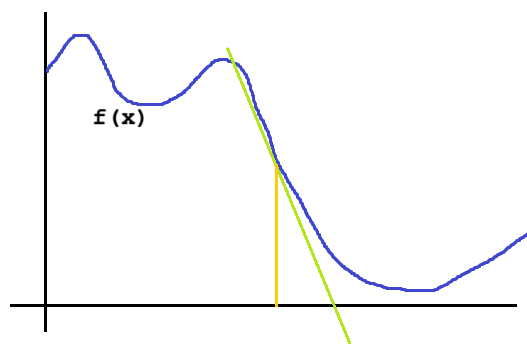
\includegraphics[width=8.5cm,keepaspectratio]{images/fx_example_01.png}
    \caption{A continuous function f defined on $\mathbb{R}$ }
    \label{contfunctionR}
\end{figure}
Assume that f is also differentiable with derivative $f'(x)$.\\
We also have a starting point $x_0$.\\
Then we get $x_1$ by subtracting $f'(x_0) \cdot \alpha$ from x, where $\alpha$ is called the learning rate, which we can choose before doing this procedure.\\
Usual values for $\alpha$ are $0.01$ or $0.05$.\\
We iterate this, so that we get an array which is recursively defined as:\\
\[x_{k+1} = x_k - f'(x_k) \cdot \alpha\]

This array will converge to the minimum of f.
The pitchfalls here are, that the procedure may end in a local minimum, while f has a stronger minimum elsewhere.\\
Or with a less than optimal choice for the learning rate, the array could even diverge.

\subsection{Gradient descent with two or more variables}
\label{GradientDescent2}
With a function $f(x, y)$ of more variables, we can determine the gradient:
\[
\nabla f(x,y) = \left( \frac{\partial f}{\partial x}, \frac{\partial f}{\partial y} \right)
\]
The method is the same, but where we took the derivative for one variable, we will now take the gradient, and the recursive definition of our array  $(x_k,y_k)$ becomes:\\
\[(x_{k+1},y_{k+1}) = (x_k,y_k) - \nabla f(x,y) \cdot \alpha\]


\subsection{Newton's method with one variable}
\label{Newton1}
Newton's method finds the zeroes of a function f. Because we're interested in finding a minimum of f,
Newton's method will help us find the zero of it's derivative $f'$ (fig \ref{NewtonMethodFig}).\\
\begin{figure}[H]
    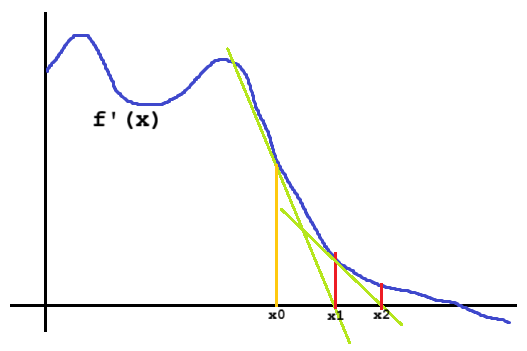
\includegraphics[width=8.5cm,keepaspectratio]{images/fx_example_02.png}
    \caption{Newton's method}
    \label{NewtonMethodFig}
\end{figure}
Geometrically, when you have the graph of f, and you have a starting point $x_0$, we start by drawing the tangent line.\\
Then we see where this tangent line intersects with the x-axis. That will be $x_1$.\\
By iterating this procedure we get an array $(x_k)_{k=0,1,\ldots}$.

From the geometrical aspect of the procedure, we can give a formula between $x_{k+1}$ and $x_k$:
\[
x_{k+1} = x_k - (f'(x_k) / f''(x_k))
\]
(that is for finding the zero of $f'$)
The idea is that the array $(x_k)$ converges to the value x where $f'(x) = 0$.\\

In order to know if $f'(x)$ points to a minimum of f, we need to look at the second derivative $f''(x)$:\\
$f''(x) > 0 \Rightarrow$ f has a minimum at x\\
$f''(x) < 0 \Rightarrow$ f has a maximum at x\\
$f''(x) = 0 \Rightarrow$ inconclusive, perhaps an inflection point\\

\subsection{Hessian matrix}
\label{HessianMatricesSub}
As explained in section \ref{GradientDescent1} the derivative of a function determines the slope of the tangent line. When the slope is positive the value of the function is increasing and when it is negative the value of the function is decreasing. When the slope is 0 the value of the function is neither rising nor decreasing. This means for this point the function has reached a maximum or minimum value.

To determine whether the found extreme is a maximum or a minimum we can use the curvature of the function. This curvature can be calculated using the second order derivative (the derivative of the derivative). When the value is negative at the extreme, the extreme is a maximum when the second derivatie is negative, it is a minimum when the second derivative is positive. When it is zero no conclusion can be made about the kind of extreme.

This knwolegde can be used, together with the Newton Method, to find minima and maxima for multi variable functions. To be sure that you only find the minimum, the second order derivative must be positive. To determine this, a Hessian matrix is constructed. The Hessian matrix contains all the second order derivates for all combinations of the variables.

Say we have function $f(x,y)$ of 2 variables.\\

Then here we have it's Hessian matrix:
\[
H_f(x,y) =
\begin{pmatrix}
\frac{\partial^2 f}{\partial x^2} & \frac{\partial^2 f}{\partial x \partial y} \\[1em]
\frac{\partial^2 f}{\partial y \partial x} & \frac{\partial^2 f}{\partial y^2}
\end{pmatrix}.
\]

A concrete example for the function $f(x) = x^3+y^3+2xy$.
The first order derivates are:\\

\begin{tabular}{l{3,5cm}l{3cm}}
\( \frac{\partial f}{\partial x} = 3x^2 + 2y \) & \( \frac{\partial f}{\partial y} = 3y^2 + 2x \) \\
\end{tabular}
\\
\\
The second order derivatives are:
\\
\\
\begin{tabular}{l{3,5cm}l{3cm}}
\( \frac{\partial^2 f}{\partial x^2} = 6x \) &\( \frac{\partial^2 f}{\partial x \partial y} = 2 \) \\
\( \frac{\partial^2 f}{\partial y \partial x} = 2 \) &\( \frac{\partial^2 f}{\partial y^2} = 6y \)
\end{tabular}
\\
\\

This creates the following Hessian Matrix:
\[
H = \begin{bmatrix}
\frac{\partial^2 f}{\partial x^2} & \frac{\partial^2 f}{\partial x \partial y} \\
\frac{\partial^2 f}{\partial y \partial x} & \frac{\partial^2 f}{\partial y^2}
\end{bmatrix}
= \begin{bmatrix}
6x & 2 \\
2 & 6y
\end{bmatrix}
\]

NU DE EIGENWAARDE


 
\subsection{Newton's method with two or more variables}
\label{Newton2}

Say we have function $f(x,y)$ of 2 variables.\\

Then here we have it's Hessian matrix:
\[
H_f(x,y) =
\begin{pmatrix}
\frac{\partial^2 f}{\partial x^2} & \frac{\partial^2 f}{\partial x \partial y} \\[1em]
\frac{\partial^2 f}{\partial y \partial x} & \frac{\partial^2 f}{\partial y^2}
\end{pmatrix}.
\]
Now at a given point (x,y) we'll calculate it's eigenvalues $\lambda_1, \lambda_2, \ldots$\\
(A 2 by 2 matrix would have at most two eigenvalues)\\

If the gradient has value (0,0) at point (x,y) then:
\begin{itemize}
    \item If all the eigenvalues of $H_f$ at (x,y) are positive, it's a minimum
    \item If all the eigenvalues of $H_f$ at (x,y) are negative, it's a maximum
    \item In other cases, it's inconclusive
\end{itemize}

In Newton's method generalized to more than one variables, the formula for the next point is:\\
\[
(x_{k+1},y_{k+1}) = (x_k,y_k) - ( H_f^{-1}(x_k,y_k) \cdot \nabla f(x_k,y_k) )
\]

\subsection{Example of a function of two variables}
\label{Example2}
We will look at this function (fig \ref{3Dsurface}):
\[
f(x,y) = 85 - \frac{1}{90}x^2(x-6)y^2(y-6)
\]
\begin{figure}[H]
    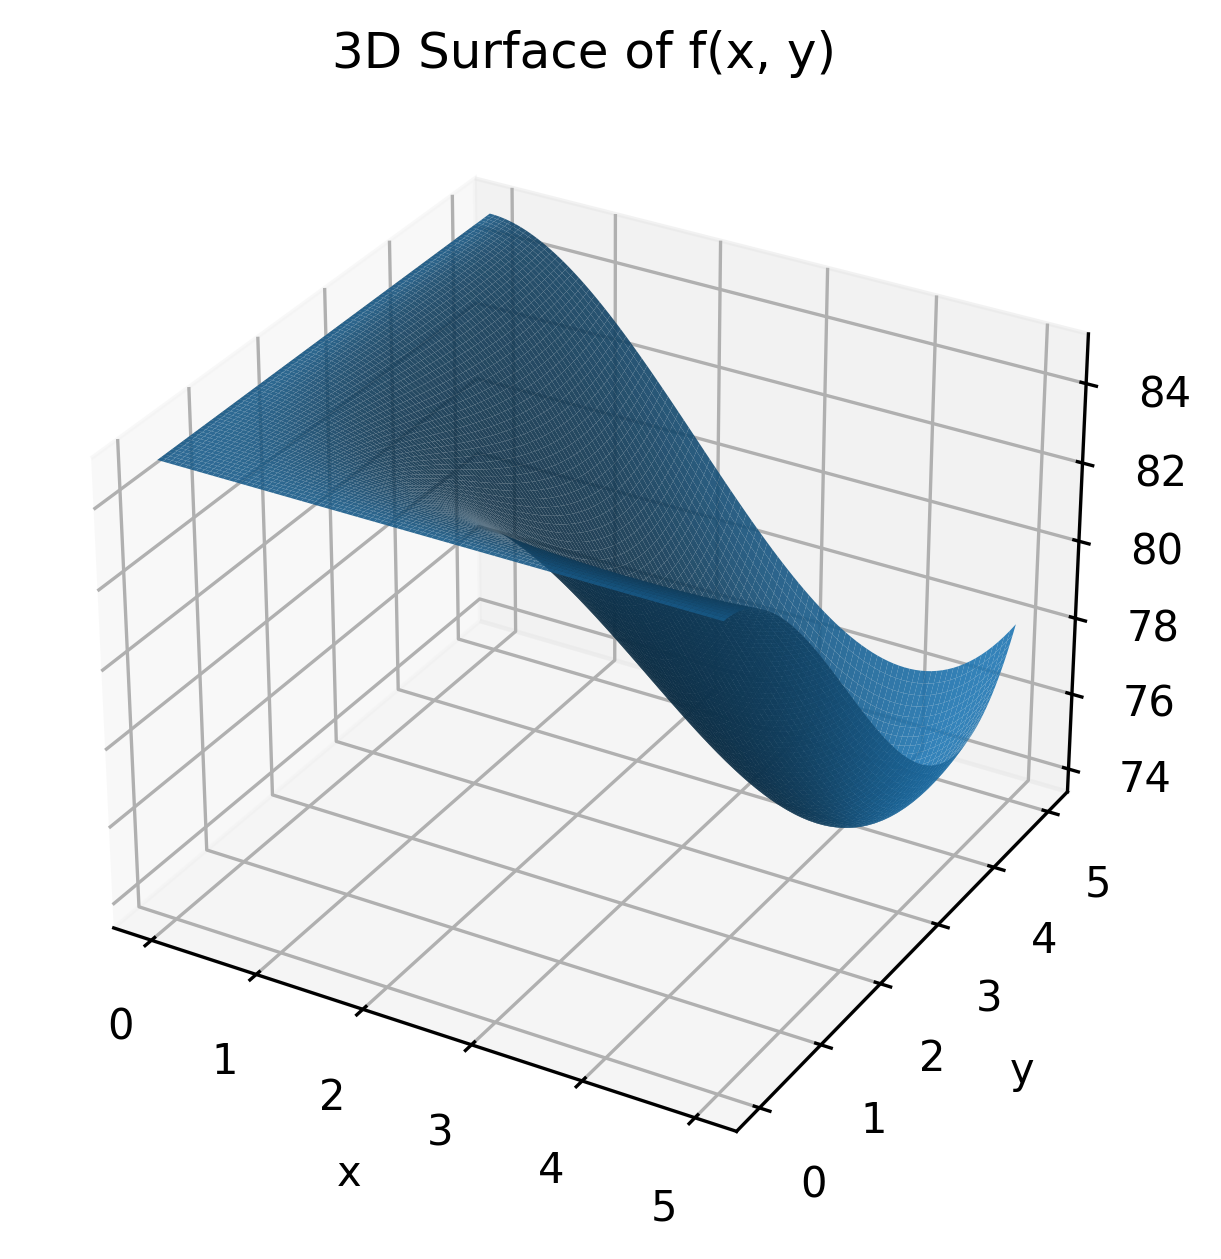
\includegraphics[width=8.5cm,keepaspectratio]{images/3D_plot.png}
    \caption{3D surface of $f(x,y)$}
    \label{3Dsurface}
\end{figure}
Visually we see a possible minimum near point $(x,y) = (4,4)$.
We'll take $(x_0,y_0) = (1,1)$ and $\alpha = 0.01$ and from there, carry out gradient descent as actual example.\\

For gradient descent, we know that we need the formula for the gradient:

$$
\nabla f(x,y) =
$$
$$
\left( - \frac{1}{90}(3x^2-12x)y^2(y-6), - \frac{1}{90}x^2(x-6)(3y^2-12y) \right)
$$
When we fill in x=1 and y=1 we calculate a gradient of (-0.5, -0.5).\\
We subtract this, multiplied by the learning rate, from (0, 0) and go to the next iteration.\\
Here we continued with a Python script that produced the following output:\\

{\footnotesize
\begin{verbatim}
0. x 1 y 1 --> (-0.500000000000000,-0.500000000000000)
1. x 1.00500000000000 y 1.00500000000000 --> (-0.506184974895937,-0.506184974895937)
2. x 1.01006184974896 y 1.01006184974896 --> (-0.512483652519824,-0.512483652519824)
3. x 1.01518668627416 y 1.01518668627416 --> (-0.518898669704649,-0.518898669704649)
...
246. x 3.98976321048153 y 3.98976321048153 --> (-0.0435643360994635,-0.0435643360994638)
247. x 3.99019885384252 y 3.99019885384252 --> (-0.0417150068300141,-0.0417150068300138)
248. x 3.99061600391082 y 3.99061600391082 --> (-0.0399437948089941,-0.0399437948089938)
249. x 3.99101544185891 y 3.99101544185891 --> (-0.0382474329314844,-0.0382474329314846)
\end{verbatim}
}
We see (x,y) approach (4,4) and we see the gradient approach (0,0). It takes 249 iterations.
We also tried learning rate 0.05. Then we saw the same behaviour, but only 56 iterations.
A tolerance of 1e-4 was used for comparing floats.

Now we will try to find the minimum using Newton's method. For this we need the second order derivatives:\\
\[
\frac{\partial^2 f}{\partial x^2} = - \frac{1}{90}(6x-12)y^2(y-6)
\]
\[
\frac{\partial^2 f}{\partial x \partial y} = - \frac{1}{90}(3x^2-12x)(3y^2-12y)
\]
\[
\frac{\partial^2 f}{\partial y \partial x} = - \frac{1}{90}(3x^2-12x)(3y^2-12y)
\]
\[
\frac{\partial^2 f}{\partial y^2} = - \frac{1}{90}x^2(x-6)(6y-12)
\]

We implemented the steps above in a python script and saw the following output:
{\footnotesize
\begin{verbatim}
(1.0000,1.0000) - (0.4054,0.4054) = (0.5946,0.5946)
(0.5946,0.5946) - (0.2190,0.2190) = (0.3756,0.3756)
(0.3756,0.3756) - (0.1327,0.1327) = (0.2429,0.2429)
(0.2429,0.2429) - (0.0839,0.0839) = (0.1589,0.1589)
(0.1589,0.1589) - (0.0542,0.0542) = (0.1047,0.1047)
(0.1047,0.1047) - (0.0354,0.0354) = (0.0693,0.0693)
(0.0693,0.0693) - (0.0233,0.0233) = (0.0460,0.0460)
(0.0460,0.0460) - (0.0154,0.0154) = (0.0305,0.0305)
(0.0305,0.0305) - (0.0102,0.0102) = (0.0203,0.0203)
(0.0203,0.0203) - (0.0068,0.0068) = (0.0135,0.0135)
(0.0135,0.0135) - (0.0045,0.0045) = (0.0090,0.0090)
(0.0090,0.0090) - (0.0030,0.0030) = (0.0060,0.0060)
(0.0060,0.0060) - (0.0020,0.0020) = (0.0040,0.0040)
(0.0040,0.0040) - (0.0013,0.0013) = (0.0027,0.0027)
(0.0027,0.0027) - (0.0009,0.0009) = (0.0018,0.0018)
(0.0018,0.0018) - (0.0006,0.0006) = (0.0012,0.0012)
(0.0012,0.0012) - (0.0004,0.0004) = (0.0008,0.0008)
(0.0008,0.0008) - (0.0003,0.0003) = (0.0005,0.0005)
(0.0005,0.0005) - (0.0002,0.0002) = (0.0004,0.0004)
(0.0004,0.0004) - (0.0001,0.0001) = (0.0002,0.0002)
(0.0002,0.0002) - (0.0001,0.0001) = (0.0002,0.0002)

Hessian from last iteration: [[-4.37584933e-08 -8.75203986e-08]
 [-8.75203986e-08 -4.37584933e-08]]
Eigenvalues of Hessian: [-1.31278892e-07  4.37619053e-08]
\end{verbatim}
}
This converges to point (0,0). The eigenvalues of the Hessian are almost zero.
So Newton's method brings us from (1,1) to a stationary point (0,0) which is not a minimum.
This happened from many other points. When we choose a starting point real close to (4,4) only then it will converge to our expected minimum:

{\footnotesize
\begin{verbatim}
(3.2000,3.2000) - (-1.4933,-1.4933) = (4.6933,4.6933)
(4.6933,4.6933) - (0.7598,0.7598) = (3.9336,3.9336)
(3.9336,3.9336) - (-0.0677,-0.0677) = (4.0013,4.0013)
(4.0013,4.0013) - (0.0013,0.0013) = (4.0000,4.0000)
(4.0000,4.0000) - (0.0000,0.0000) = (4.0000,4.0000)

Hessian from last iteration: [[ 4.26666750e+00 -2.45347276e-13]
 [-2.45347276e-13  4.26666750e+00]]
Eigenvalues of Hessian: [4.2666675 4.2666675]
\end{verbatim}
}
The point reached here is indeed (4,4). The eigenvalues of the Hessian are positive, and indeed this is in line with that we already know,
that (4,4) is a minimum.\\
From (3.2,3.2) it took 5 iterations. When we try Gradient Descent from this point (3.2,3.2) we will see the number of iterations for that:
{\footnotesize
\begin{verbatim}
Gradient Descent from (3.2,3.2) with learning rate 0.01 takes 109 iterations to reach (4,4).
Gradient Descent from (3.2,3.2) with learning rate 0.05 takes 27 iterations to reach (4,4).
\end{verbatim}
}



\subsection{Hessian Matrices}
\label{HessianMatrices}





\printbibliography


% that's all folks
\end{document}


